
% xetex expected
\documentclass[xetex,professionalfont]{beamer}

% we want math
\usepackage{amsmath}

% fixes and extensions to amsmath
\usepackage{mathtools}

% additional math symbols
\usepackage{amssymb}

% good-looking fractions in text via \sfrac
\usepackage{xfrac}

% fix spaces after custom commands (see below for examples)
\usepackage{xspace}

% minted allows for fancy syntax highlighting (requires python with pygments)
% usage:
%   \begin{minted}{python}
%   codeb
%   \end{minted}
\usepackage{minted}

% better looking tables
% usage:
%   begin with a \toprule, write a single row of column headings,
%   then add \midrule and after the columns of data we finish with \bottomrule
% example:
%   \begin{tabular}{llr} \toprule
%   Animal & Description & Price \midrule
%   cat & foo & 10 \\
%   dog & bar & 20 \\ \bottomrule
%   \end{tabular}
% note that good tables generally neither have vertical rules nor double rules
\usepackage{booktabs}

% system font support (requires xetex or luatex)
\usepackage{fontspec}
\setmonofont[Scale=0.7]{Cousine} % part of ttf-chromeos fonts on Arch

% improve microtypography
\usepackage{microtype}

% multi-language quotes for babel
\usepackage{csquotes}

% easy way to include copyright information
\usepackage{copyrightbox}

% better bibliographies
\usepackage[backend=biber,style=authoryear]{biblatex}

% language support (english,ngerman)
\usepackage[english]{babel}

% plots (part of texlive-pictures)
\usepackage{pgfplots}

% process diagrams (part of texlive-pictures)
\usepackage{smartdiagram}

% diagram style

\smartdiagramset{norm/.style={
     sequence item border color=gray!30!black,
     sequence item border size=1.5\pgflinewidth,
     sequence item font size=\footnotesize,
  }
}

\smartdiagramset{transp/.style={
     sequence item border color=gray!70!black,
     sequence item border size=1.5\pgflinewidth,
     sequence item font size=\footnotesize,
     sequence item fill opacity=0.5,
     sequence item text opacity=0.5
  }
}

\smartdiagramset{norm}

% -----------------------------------------------------------------------------

% specify PDF metadata
\hypersetup{pdftitle={CVSP VO - Object Recognition},pdfsubject={},pdfauthor={Christopher Pramerdorfer}}

% copyright font style
\makeatletter\renewcommand{\CRB@setcopyrightfont}{\tiny\color{lightgray}}

% make emph bold
\DeclareTextFontCommand{\emph}{\bfseries}

% use tuwcvl beamer theme
\usetheme{tuwcvl}

% add bib file
\addbibresource{literature.bib}

% plot setup

\pgfplotsset{width=6.5cm,compat=1.11}

\definecolor{darkgreen}{rgb}{0,0.8,0.1}

% -----------------------------------------------------------------------------

% common english abbreviations
\newcommand{\ie}{\mbox{i.e.}\xspace} % i.e.
\newcommand{\eg}{\mbox{e.g.}\xspace} % e.g.
\newcommand{\wrt}{\mbox{wrt.}\xspace} % wrt.

% math - argmin and argmax
\DeclareMathOperator*{\argmin}{arg\,min}
\DeclareMathOperator*{\argmax}{arg\,max}

\DeclareMathOperator*{\Norm}{Norm}
\DeclareMathOperator*{\Uniform}{Uniform}
\DeclareMathOperator*{\Bern}{Bern}

% shortcuts for number ranges
\newcommand{\NN}{\mathbb{N}}
\newcommand{\ZZ}{\mathbb{Z}}
\newcommand{\QQ}{\mathbb{Q}}
\newcommand{\RR}{\mathbb{R}}

% bold vectors
\renewcommand{\vec}[1]{\ensuremath{\mathbf{#1}}}

% vector shortcuts
\newcommand{\va}{\vec{a}}
\newcommand{\vb}{\vec{b}}
\newcommand{\vc}{\vec{c}}
\newcommand{\ve}{\vec{e}}
\newcommand{\vr}{\vec{r}}
\newcommand{\vs}{\vec{s}}
\newcommand{\vt}{\vec{t}}
\newcommand{\vu}{\vec{u}}
\newcommand{\vv}{\vec{v}}
\newcommand{\vw}{\vec{w}}
\newcommand{\vx}{\vec{x}}
\newcommand{\vy}{\vec{y}}
\newcommand{\vz}{\vec{z}}
\newcommand{\vp}{\vec{p}}
\newcommand{\vq}{\vec{q}}
\newcommand{\vn}{\vec{n}}

% bold greek symbols
\newcommand{\bth}{\boldsymbol{\theta}}
\newcommand{\intr}{\boldsymbol{\Lambda}}
\newcommand{\trans}{\mathcal{T}}

% -----------------------------------------------------------------------------

\title{Computer Vision Systems Programming VO}
\subtitle{Object Recognition}
\author{Christopher Pramerdorfer}
\institute{Computer Vision Lab, Vienna University of Technology}

\begin{document}

% -----------------------------------------------------------------------------

\begin{frame}
\maketitle
\end{frame}

% -----------------------------------------------------------------------------

\begin{frame}
\frametitle{Topics}

Selection of recognition problems
\begin{itemize}
    \item Detecting specific rigid objects
    \item Efficient face detection
    \item Image classification
\end{itemize}

\bigskip
\begin{center}
    \copyrightbox[b]
    {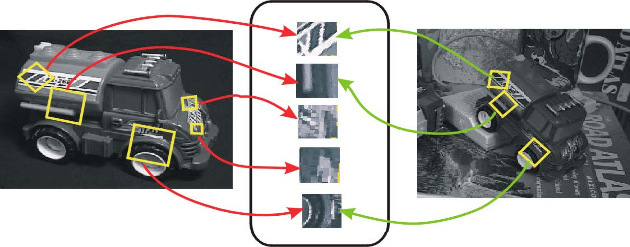
\includegraphics[width=6.5cm]{figures/local-feature-matching.jpg}}
    {\centering Image from \cite{grauman2011}}
\end{center}

\end{frame}

% -----------------------------------------------------------------------------

\begin{frame}
\frametitle{Taxonomy of Object Recognition}

Instance vs.\ category recognition
\begin{itemize}
    \item Instance : my face, the Eiffel tower
    \item Category : faces, buildings, people % note that categories are hierarchical ... like panda bears - bears - mammals - animals. some test databases reflect this, like ImageNet. obviously, the more general the category, the harder the recognition task
\end{itemize}

\bigskip
Classification vs.\ detection
\begin{itemize}
    \item Classification : predict class of main object in image % here we assume that there is a dominant object in the image, and we care only about the class (instance/category) of that object, ignoring the rest
    \item Detection : multiple objects, possibly of different class % like "detect all faces in image"
\end{itemize}

\end{frame}

% -----------------------------------------------------------------------------

\begin{frame}
\frametitle{Taxonomy of Object Recognition}
\framesubtitle{Classification}

Blue Mosque (instance), mosque/building (category) % again, categories are hierarchical

\bigskip
\begin{center}
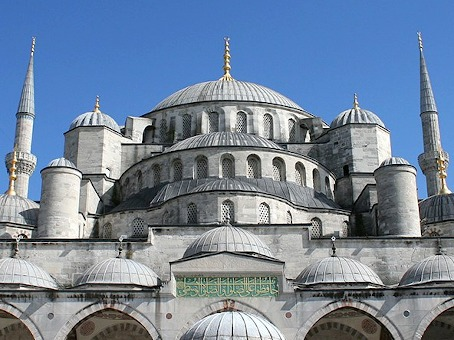
\includegraphics[width=6cm]{figures/blue-mosque.jpg}
\end{center}

\end{frame}

% -----------------------------------------------------------------------------

\begin{frame}
\frametitle{Taxonomy of Object Recognition}
\framesubtitle{Detection}

\begin{center}
    \copyrightbox[b]
    {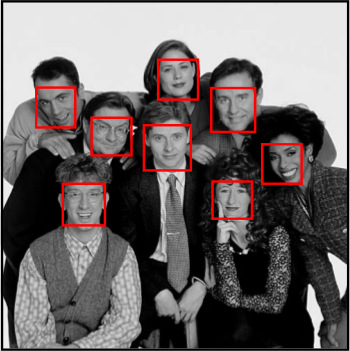
\includegraphics[width=5cm]{figures/face-detection.jpg}}
    {\centering Image from \cite{prince12}}
\end{center}

\end{frame}

% -----------------------------------------------------------------------------

\begin{frame}
\frametitle{Challenges}

Instances of same category can look very differently
\begin{itemize}
    \item Illumination, pose, viewpoint, occlusions, background
\end{itemize}

\begin{center}
    \copyrightbox[b]
    {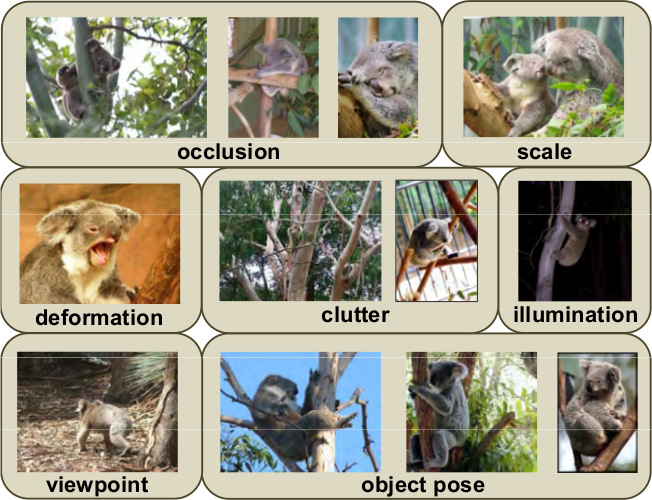
\includegraphics[width=5.5cm]{figures/challenges.jpg}}
    {\centering Image from \cite{grauman2011}}
\end{center}

\end{frame}

% -----------------------------------------------------------------------------

\begin{frame}
\frametitle{Detecting Specific Rigid Objects} % this is obviously an instance recognition problem

\begin{center}
    \copyrightbox[b]
    {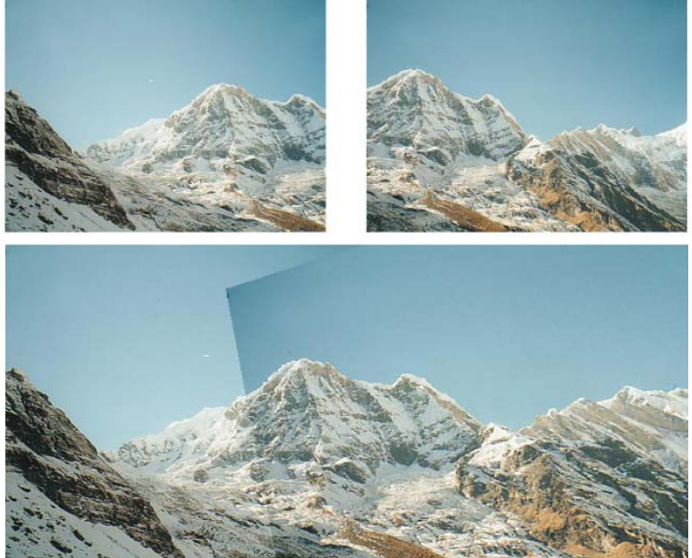
\includegraphics[width=7cm]{figures/panorama-stitching.jpg}} % stitching is not the typical example, but it can be seen as one
    {\centering Image adapted from \cite{brown2007}}
\end{center}

\end{frame}

% -----------------------------------------------------------------------------

\begin{frame}
\frametitle{Detecting Specific Rigid Objects}

Often accomplished via \emph{local feature matching}

\bigskip
Given an image of the object and a search image
\begin{itemize}
    \item Compute local features in both images
    \item Match features between images to find correspondences
    \item Perform geometric verification % this is possible due to rigidity
\end{itemize}

\end{frame}

% -----------------------------------------------------------------------------

\begin{frame}
\frametitle{Detecting Specific Rigid Objects}
\framesubtitle{Local Feature Representations}

Local features form a sparse object representation
\begin{itemize}
    \item Features capture characteristic structure
    \item Allow for efficient matching between images
    \item Representation robust to occlusion and clutter % due to the local features
\end{itemize}

\begin{center}
    \copyrightbox[b]
    {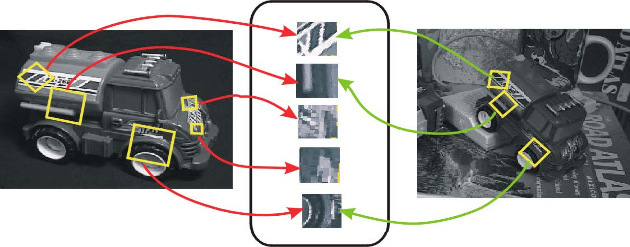
\includegraphics[width=8cm]{figures/local-feature-matching.jpg}}
    {\centering Image from \cite{grauman2011}}
\end{center}

\end{frame}

% -----------------------------------------------------------------------------

\begin{frame}
\frametitle{Detecting Specific Rigid Objects}
\framesubtitle{Local Feature Representations}

Many different feature extractors available
\begin{itemize}
    \item SIFT, SURF, BRISK, FREAK, ... % we have covered SIFT shortly in a previous lecture. no more coverage here on the other ones, but they are all quite similar
    \item OpenCV includes implementations
\end{itemize}

\bigskip
Guidelines on feature selection
\begin{itemize}
    \item Features should be invariant to expected transformations % like rotation, scale, affine transforms
    \item And only to these transformations
    \item Extraction and matching speeds differ % not a problem if object should be searched for in 5 images, but what if in 1000 images? (if there are more, we at some point have to switch to more efficient means, like hashing or vector quantization (like what we do later with visual words))
    \item Performance often quite similar, but better test % there are also some survey papers around
\end{itemize}

\end{frame}

% -----------------------------------------------------------------------------

\begin{frame}
\frametitle{Detecting Specific Rigid Objects}
\framesubtitle{Feature Matching}

Features are $n$-dimensional vectors
\begin{itemize}
    \item Perform nearest neighbor matching in this feature space
\end{itemize}

\bigskip
Popular matching strategy
\begin{itemize}
    \item Given feature $\vx$ in first image
    \item Find two nearest neighbors $\vy_1,\vy_2$ from second image
    \item $\{\vx,\vy_1\}$ correspond if $\lVert\vx-\vy_1\rVert/\lVert\vx-\vy_2\rVert<0.8$ % y2 is further away from x as y1, hence this fraction is always below 1. the smaller the fraction the smaller the match ambiguity, hence this matching strategy eliminates most false matches / note that this is the Euclidean distance if features in R^n. newer features often use binary descriptors, in which case the Hamming distance is often used for comparison. but this matching strategy still applies
\end{itemize}

\end{frame}

% -----------------------------------------------------------------------------

\begin{frame}
\frametitle{Detecting Specific Rigid Objects}
\framesubtitle{Geometric Verification}

Assume that the object in question is planar
\begin{itemize}
    \item Images of planar objects are related by a homography % for nonplanar scenes this is only the case if the camera only zooms or rotates around the center of projection
    \item Also applies to local feature locations
\end{itemize}

\smallskip
\begin{center}
    \copyrightbox[b]
    {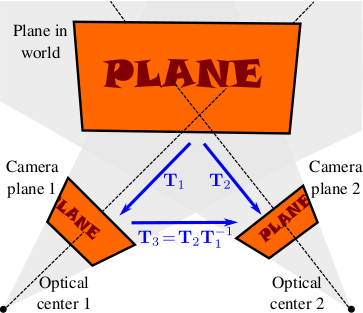
\includegraphics[width=4.5cm]{figures/planar-homography}}
    {\centering Image from \cite{prince12}}
\end{center}

\end{frame}

% -----------------------------------------------------------------------------

\begin{frame}
\frametitle{Detecting Specific Rigid Objects}
\framesubtitle{Geometric Verification}

Relation allows for detecting erroneous correspondences
\begin{itemize}
    \item Estimate homography $T$ from correspondences % using some robust method, like RANSAC
    \item Discard correspondences for which $\lVert\vx-T(\vy_1)\rVert>t$ % if x and y1 really correspond, their projections must lie close together ... t is some small threshold that depends on the data, usually a few pixels
\end{itemize}

\bigskip
Verification also possible for nonplanar scenes
\begin{itemize}
    \item Epipolar geometry constraints (previous lecture) % basically, if we know the intrinsics we can estimate the relative camera positions/orientations, which is all we need as discussed in the previous lecture. if we dont know the intrinsics, this is still possible by computing the fundamental matrix. this is out of scope here, but see any of the CV books referenced below if interested
\end{itemize}

\end{frame}

% -----------------------------------------------------------------------------

\begin{frame}[fragile]
\frametitle{Detecting Specific Rigid Objects}
\framesubtitle{OpenCV Code Example}

\footnotesize
\begin{minted}{cpp}
// read images (SIFT expects grayscale images)
cv::Mat object = cv::imread("object.jpg", cv::IMREAD_GRAYSCALE);
cv::Mat search = cv::imread("search.jpg", cv::IMREAD_GRAYSCALE);

cv::SIFT sift; // using default arguments here

// compute keypoints
std::vector<cv::KeyPoint> kobject, ksearch;
sift.detect(object, kobject); sift.detect(search, ksearch);

// compute descriptors (our x, y)
cv::Mat dobject, dsearch;
sift.compute(object, kobject, dobject); sift.compute(search, ksearch, dsearch);
\end{minted}

\end{frame}

% -----------------------------------------------------------------------------

\begin{frame}[fragile]
\frametitle{Detecting Specific Rigid Objects}
\framesubtitle{OpenCV Code Example}

\footnotesize
\begin{minted}{cpp}
// find y1,y2 for each x
cv::FlannBasedMatcher matcher; // fast nearest neighbor search
std::vector<std::vector<cv::DMatch> > kMatches;
matcher.knnMatch(dobject, dsearch, kMatches, 2);

// select good matches (see above slide)
std::vector<cv::DMatch> matches;
for(const std::vector<cv::DMatch>& match : kMatches)
    if(match[0].distance < match[1].distance * 0.8)
        matches.push_back(match[0]); // (x,y1)
\end{minted}

\end{frame}

% -----------------------------------------------------------------------------

\begin{frame}[fragile]
\frametitle{Detecting Specific Rigid Objects}
\framesubtitle{OpenCV Code Example}

\footnotesize
\begin{minted}{cpp}
// collect feature locations of correspondences
std::vector<cv::Point2f> pobject, psearch;
for(const cv::DMatch& match : matches) { 
    pobject.push_back(kobject.at(match.queryIdx).pt);
    psearch.push_back(ksearch.at(match.trainIdx).pt);
}

// estimate homography using RANSAC for robustness
cv::Mat inliers; // contains indices of valid correspondences
cv::Mat homography = cv::findHomography(pobject, psearch, CV_RANSAC, 3, inliers);
\end{minted}

\end{frame}

% -----------------------------------------------------------------------------

\begin{frame}
\frametitle{Detecting Specific Rigid Objects}
\framesubtitle{Applications -- Object Detection}

Detection and 2D pose estimation

\bigskip
\begin{center}
    \copyrightbox[b]
    {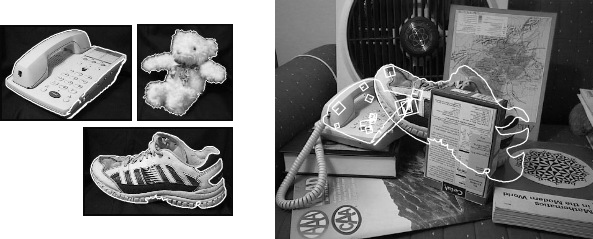
\includegraphics[width=8cm]{figures/rigid-object-detection.jpg}} % note the occlusions and transformations
    {\centering Image adapted from \cite{lowe2004}}
\end{center}

\end{frame}

% -----------------------------------------------------------------------------

\begin{frame}
\frametitle{Detecting Specific Rigid Objects}
\framesubtitle{Applications -- Object Detection}

Industrial applications like PCB recycling

\bigskip
\begin{center}
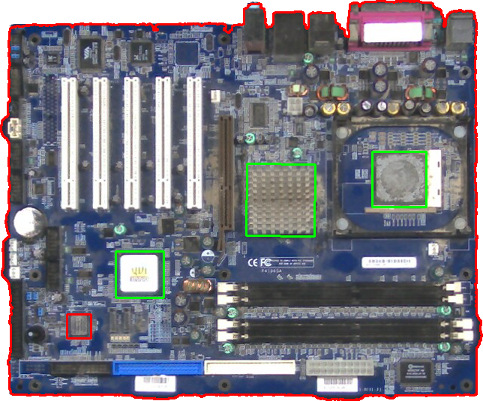
\includegraphics[width=5.5cm]{figures/reclaim-pcb.jpg}
\end{center}

\end{frame}

% -----------------------------------------------------------------------------

\begin{frame}
\frametitle{Detecting Specific Rigid Objects}
\framesubtitle{Applications -- Panorama Stitching}

\begin{center}
    \copyrightbox[b]
    {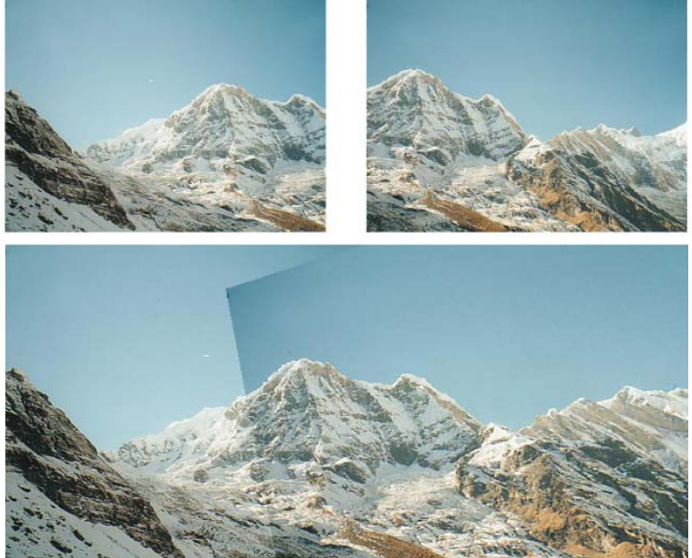
\includegraphics[width=7cm]{figures/panorama-stitching.jpg}}
    {\centering Image adapted from \cite{brown2007}}
\end{center}

\end{frame}

% -----------------------------------------------------------------------------

\begin{frame}
\frametitle{Efficient Face Detection} % this is a category recognition problem

\begin{center}
    \copyrightbox[b]
    {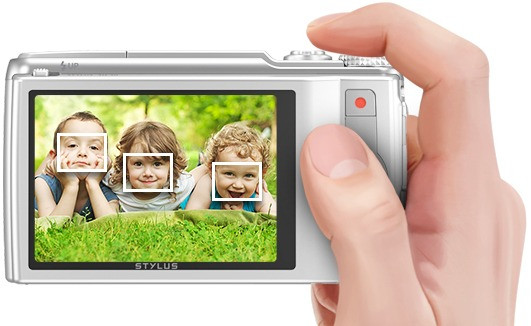
\includegraphics[width=7cm]{figures/camera-faces.jpg}}
    {\centering Image from \url{olympus-europa.com}}
\end{center}

\end{frame}

% -----------------------------------------------------------------------------

\begin{frame}
\frametitle{Efficient Face Detection}

Face detection has many applications, such as
\begin{itemize}
    \item Smart cameras (autofocus on faces)
    \item Security (preprocessing step to face recognition)
    \item Augmented reality \& gaming
\end{itemize}

\bigskip
We focus on the popular method from [\cite{viola2001}]
\begin{itemize}
    \item Fast enough to run on e.g.\ cameras
\end{itemize}

\end{frame}

% -----------------------------------------------------------------------------

\begin{frame}
\frametitle{Efficient Face Detection}

Sliding window approach % we don't know where the faces might be, so we just scan over the whole image. note that the window size depends on the expected size of the faces, and as such is not scale invariant (but we could repeat the test with different scales)
\begin{itemize}
    \item Slide window over image % note that this results one classification per pixel (unless we chose some offset), and the classification is binary ... w denotes whether a face is present
    \item Infer label $w\in\{0,1\}$ based on measurements $\vx$ % of the current window
    \item Perform non-maximum suppression of confidence scores % we also get some form of confidence along with the label (similar to the probabilistic models we discussed, but they are not probabilities)
\end{itemize}

\medskip
\begin{center}
\begin{tikzpicture}
\node [inner sep=0pt,above right]{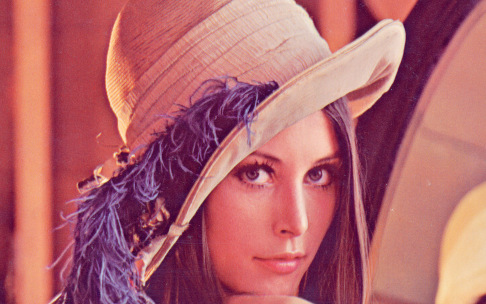
\includegraphics[width=5cm]{figures/lena.jpg}};;
\draw[thick,green,opacity=0.2] (1.6,0.25) rectangle (3.6,2.25);
\draw[thick,green,opacity=0.4] (1.7,0.25) rectangle (3.7,2.25);
\draw[thick,green,opacity=0.6] (1.8,0.25) rectangle (3.8,2.25);
\draw[thick,green,opacity=0.8] (1.9,0.25) rectangle (3.9,2.25);
\draw[thick,green] (2,0.25) rectangle (4,2.25);
\end{tikzpicture}
\end{center}

\end{frame}

% -----------------------------------------------------------------------------

\begin{frame}
\frametitle{Efficient Face Detection}

Simple features -- difference $d$ in rectangular subwindow of $\vx$
\begin{itemize}
    \item Can be computed in constant time using integral images
    \item Limited number of such features, $\{f_t\}_{t=1}^T$ % for a given window size
\end{itemize}

\bigskip
\begin{center}
    \copyrightbox[b]
    {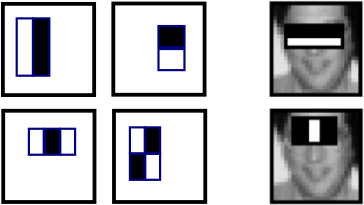
\includegraphics[width=5cm]{figures/vj-features.png}}
    {\centering Image adapted from \cite{prince12}}
\end{center}

\end{frame}

% -----------------------------------------------------------------------------

\begin{frame}
\frametitle{Efficient Face Detection}

Classification using a \emph{boosted cascade}
\begin{itemize}
    \item Cascade of $K\leq T$ weak but fast classifiers $c_k=f_k>t_k$ % K is something we can define. around 6k in the original paper
    \item Early rejection of non-face windows for speed % we just abort as soon as the patch is not classified as a face
    \item Final classifier is $C(\vx)=\text{sign}(\theta_0+\sum_k \theta_k c_k)$ % theta are some learned weights
\end{itemize}

\medskip
\begin{center}
    \copyrightbox[b]
    {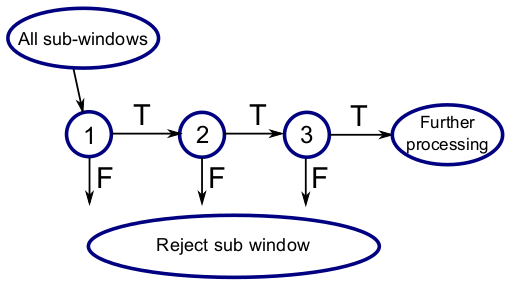
\includegraphics[width=5cm]{figures/boosting-cascade}}
    {\centering Image from \cite{prince12}}
\end{center}

\end{frame}

% -----------------------------------------------------------------------------

\begin{frame}
\frametitle{Efficient Face Detection}

Subset of $K$ best classifiers, their order, and $\bth$ are learned

\bigskip
By means of \emph{boosting} : for each $k=1\cdots K$
\begin{itemize}
    \item Find best classifier according to training set, add to $C$ % this is the classifier that, if added to the current C(x), leads to the biggest reduction in error
    \item Raise weights of samples misclassified by current $C$
\end{itemize}

\bigskip
\begin{center}
    \copyrightbox[b]
    {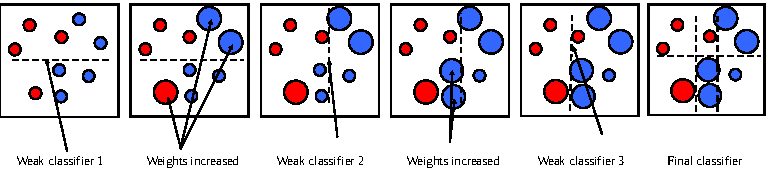
\includegraphics[width=10cm]{figures/boosting.pdf}} % see Szeliski's book for a good explanation
    {\centering Image from \cite{szeliski2010}}
\end{center}

\end{frame}

% -----------------------------------------------------------------------------

\begin{frame}[fragile]
\frametitle{Efficient Face Detection}
\framesubtitle{OpenCV Code Example}

Detect faces using a pretrained cascade\\\medskip
OpenCV also supports cascade training

\bigskip
\footnotesize
\begin{minted}{python}
# detect faces using a pretrained cascade
image = cv2.imread('faces.jpg', cv2.IMREAD_GRAYSCALE)
cascade = cv2.CascadeClassifier('haarcascade_frontalface_default.xml')
faces = cascade.detectMultiScale(image) # should tune parameters
\end{minted}

\end{frame}

% -----------------------------------------------------------------------------

\begin{frame}
\frametitle{Image Classification}

Goal is to predict the class of the main object in an image\\\medskip
We consider methods based on visual words 

\medskip
\begin{center}
    \copyrightbox[b]
    {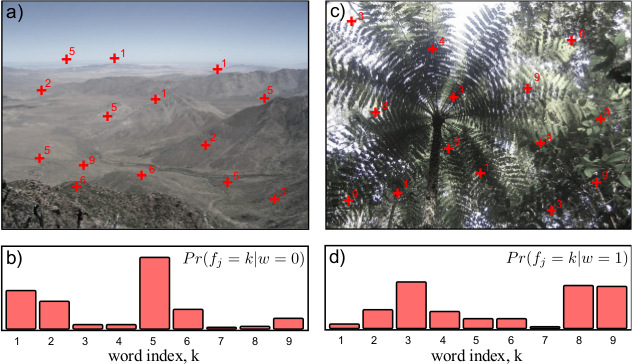
\includegraphics[width=7cm]{figures/visual-words.jpg}}
    {\centering Image from \cite{prince12}}
\end{center}

\end{frame}

% -----------------------------------------------------------------------------

\begin{frame}
\frametitle{Image Classification}

Idea is to represent an image as a collection of \emph{visual words} % this comes from document retrieval - a text consists of words, an image of visual words, so we represent an image by the distribution of its visual words
\begin{itemize}
    \item Images can be compared based on visual word distribution
\end{itemize}

\medskip
\begin{center}
    \copyrightbox[b]
    {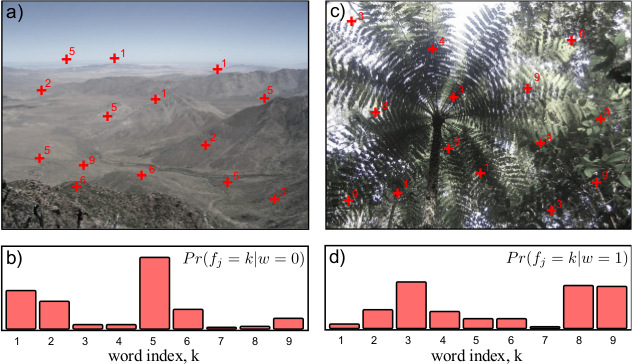
\includegraphics[width=7cm]{figures/visual-words.jpg}} % we see that the visual word representations of these images differ, so they are not of the same class
    {\centering Image from \cite{prince12}}
\end{center}

\end{frame}

% -----------------------------------------------------------------------------

\begin{frame}
\frametitle{Image Classification}

Visual words are learned from an image collection
\begin{itemize}
    \item Compute local features for all images
    \item Cluster these vectors into $k$ clusters using $k$-means % this is the standard method, can use other clustering methods as well
    \item $k$ cluster means represent visual words
\end{itemize}

\begin{center}
    \copyrightbox[b]
    {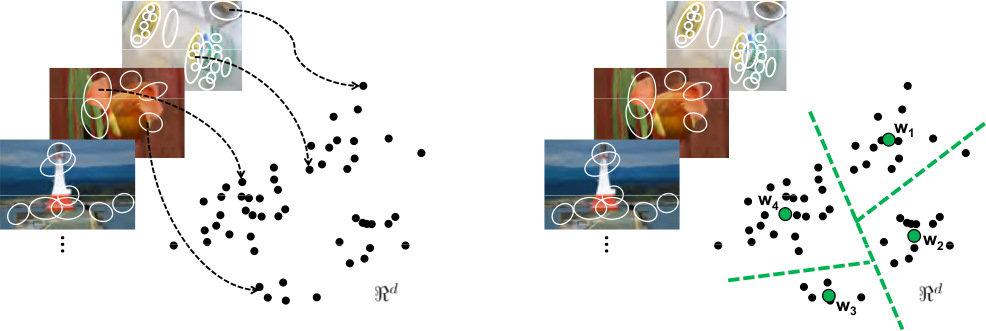
\includegraphics[width=8cm]{figures/visual-word-construction.jpg}}
    {\centering Image from \cite{grauman2011}}
\end{center}

\end{frame}

% -----------------------------------------------------------------------------

\begin{frame}
\frametitle{Image Classification}

Visual word distribution $\vx\in\RR^k$ of image obtained by
\begin{itemize}
    \item Computing local features for current image
    \item Assigning each feature to closest visual word % this is again the simplest approach, better performance can be achieved using fuzzy assignment
    \item Summing up the assignment counts for each visual word % and normalizing them of course
\end{itemize}

\begin{center}
    \copyrightbox[b]
    {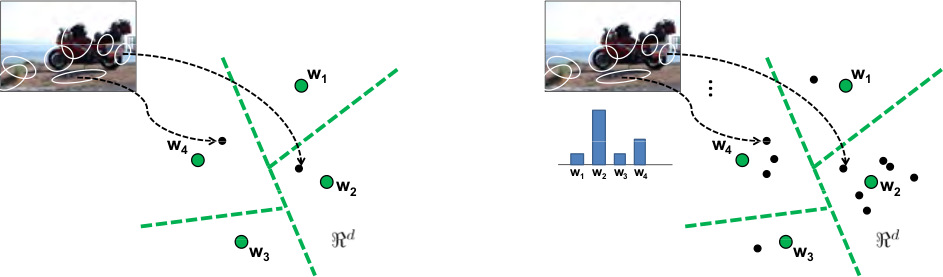
\includegraphics[width=8cm]{figures/visual-word-generation.jpg}}
    {\centering Image from \cite{grauman2011}}
\end{center}

\end{frame}

% -----------------------------------------------------------------------------

\begin{frame}
\frametitle{Image Classification}

Prediction of class $w$ from $\vx$ using e.g.\ SVM % can use anything here, but SVMs are popular in this context
\begin{itemize}
    \item Classifier learned using training samples $\{(\vx,w)\}$
\end{itemize}

\bigskip
\begin{center}
\smartdiagram[sequence diagram]{Image,Visual Words,SVM}
\end{center}

\end{frame}

% -----------------------------------------------------------------------------

\begin{frame}
\frametitle{Image Classification}

The above approach is called \emph{bag of words} model
\begin{itemize}
    \item Many improvements to this methods exist
    \item Popular and can work well, but not state of the art % tor this reason, this was quite short, basically in order to make the differences to deep learning clearer
\end{itemize}

\bigskip
We will look at the current state of the art next time

\end{frame}

% -----------------------------------------------------------------------------

\begin{frame}
\frametitle{Summary}

Object recognition is key to many successful applications

\bigskip
We have discussed three popular cases
\begin{itemize}
    \item Detecting specific rigid objects
    \item Efficient face detection
    \item Image classification from visual words
\end{itemize}

\end{frame}

% -----------------------------------------------------------------------------

\begin{frame}[allowframebreaks=0.8]
\frametitle{Bibliography}

\printbibliography

\end{frame}

\end{document}
